\chapter{Requirements}
\label{cha:requirements}

This  work deals  with  an  execution environment  that  uses Xen  virtual
machines to run  applications in a secure environment.   In this chapter I
am going to describe, how such an environment can look like and what it is
supposed to provide the users with.

\begin{figure}[htbp]
  \begin{center}
    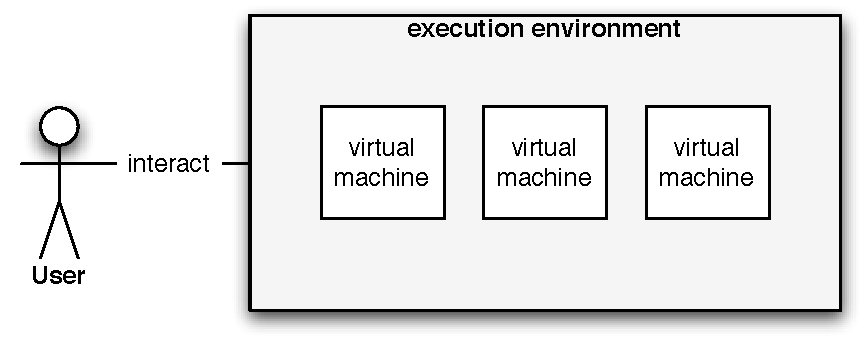
\includegraphics[scale=.5]{concept}
  \end{center}
  \caption[Conceptual overview]{A conceptual overview}
  \label{fig:concept}
\end{figure}

In Figure~\ref{fig:concept},  a conceptual overview  is shown, it  depicts a
single user interacting with the execution environment.

The next sections describe what  I think, an execution environment must at
least provide to be useful. Furthermore, several use-cases are given, that
show possible usage scenarios of the execution environment.

\section{Execution environment}
\label{sec:req-execution-environment}

What should an execution environment  provide, so that users can work with
it?  I  think  the following  list  gives  a  good  idea about  the  basic
requirements any execution environment should fulfill:

\begin{itemize}
\item \emph{Submit new tasks} --- i.e.~inform the system about a new task,
  that it should execute.
\item \emph{Query the status of  tasks} --- i.e.~is the task still pending
  and  waiting for  its execution,  currently  running or  did it  already
  finish.
\item \emph{Stop running tasks} --- i.e.~a user must always have the
  possibility to cancel his own tasks.
\end{itemize}

Typically, tasks  require some input data  to work on  and generate output
data  ---  to describe  such  tasks  we  demand the  following  additional
requirements:
\begin{itemize}
\item Provide a way to specify input data for a task
\item Provide a way to retrieve generated output data from a task
\end{itemize}

The next sections describe each point in more detail --- they also explain
specifications  such  as the  \emph{Job  Submission Description  Language}
(\gls{glo:JSDL}) \cite{jsdl-spec}  and the \emph{Basic  Execution Service}
(\gls{glo:BES}) \cite{ogsa-bes}.

\subsection{Submission of tasks}
\label{sec:req-task-submission}

In  grid environments,  for example,  the user  describes his  job  as the
application he wants to execute,  additional parameters that are passed to
the application, input and output data and many more.

The here proposed execution environment demands a way to describe not only
the tasks, but also  the virtual machine that is going to  be used for the
task.

An upcoming standard for a job description, that is not restricted to grid
environments, but  can be used  in various environments, is  the \emph{Job
  Submission  Description  Language}   ---  or  \gls{glo:JSDL}  for  short
\cite{jsdl-spec}.

I  decided to  use this  description language,  so that  the Xen-execution
environment can  easily be integrated  into various middlewares  that also
use the \gls{glo:JSDL} to describe their jobs.

\subsubsection{Job Submission Description Language (\gls{glo:JSDL})}

\gls{glo:JSDL}  is a  very extensible  XML-based description  language for
computational  jobs.  With  \gls{glo:JSDL} you  are able  to  describe all
requirements that  a computational  job may need  for the submission  to a
resource --- mainly the \gls{glo:JSDL}  addresses grid resources but it is
not limited the latter.

\paragraph{The building   blocks}

A  \gls{glo:JSDL}   document  always  contains   a  \texttt{JobDefinition}
element, which is the top-level element and holds all required information
about the job.

A  minimalistic  example is  shown  in Listing~\ref{lst:jsdl-example},  it
describes the execution of the following command in a standard UNIX shell:

\begin{minipage}{0.75\textwidth}
  \begin{lstlisting}[language=ksh]
    $ echo Hello World
    Hello World
    $
  \end{lstlisting}
\end{minipage}

\lstinputlisting[float=ht,caption={A small ``Hello World''-example written in \gls{glo:JSDL}},label={lst:jsdl-example},language=XML]{examples/jsdl-example.jsdl}

\bigskip

A typical \gls{glo:JSDL} document consists  of the following parts --- job
identification,  application description,  resource descriptions  and data
staging elements:

\begin{description}
\item[\emph{JobIdentification}] This element  is used to hold information
  about the job that is mostly  interesting for human beings --- such as a
  descriptive  name  for the  job.   Nonetheless  it  may hold  additional
  information  that  could  be  of  interest to  machines  processing  the
  document  --- such  as  annotations (e.g.~a  unique task  identification
  number can be stored in such an annotation).
\item[\emph{Application}] With this element,  a user describes the program
  itself  --- i.e.~the real  executable, that  is to  be used.   A special
  extension   ---   \texttt{POSIXApplication},   also   defined   in   the
  specification \cite{jsdl-spec}  --- can be used  to describe executables
  for    \gls{glo:POSIX}-compliant    operating   systems    \cite{posix}.
  Listing~\ref{lst:jsdl-example}   uses  this   element  to   execute  the
  \texttt{echo} program.
\item[\emph{Resources}]  This  element can  be  used  to describe  various
  resource requirements  of the  application. Some examples  for resources
  are:
  \begin{itemize}
  \item the number of CPUs the job requires
  \item the operating system required by the job
  \item amount of virtual memory that must be available for the job
  \item file-systems and their mount-points that have to be made available
    for the job
  \end{itemize}
  The file-system definitions  are placeholder variables for \emph{logical
    places} within  the file-system hierarchy.  They can be used  in other
  elements to refer to some file ``below'' a particular file-system.
\item[\emph{DataStaging}]   The   \texttt{DataStaging}   element  can   be
  specified  arbitrarily often  and  defines both  stage-in and  stage-out
  operations.   A stage-in operation  is a  file-transfer that  must occur
  prior executing  the job (i.e.~it prepares  the input data  for the job)
  and obviously stage-out operations take place after the job has finished
  its execution.

  The  most relevant  elements within  a DataStaging  instruction  are the
  \texttt{Source} and \texttt{Target} elements ---  both can hold a URI to
  specify a  generic location ---  and the \texttt{FileName} element which
  points to an actual file within the file-system hierarchy.
\end{description}

As you  can see, the \gls{glo:JSDL}  is really powerful and  it covers all
requirements  a typical computational  job may  have. And  if it  does not
cover a  special topic, one  is able to  extend the defined  elements with
custom elements.

\subsubsection{Extensions to the \gls{glo:JSDL}}

To be able to create a virtual machine on the remote site, the user has to
specify not only  the application she wants to run  but also a file-system
\gls{glo:image}  that  contains  an  operating system  installation.   The
execution environment then  takes care of starting up  the virtual machine
with  the  provided  \gls{glo:image}   and  will  eventually  execute  the
application.

The  description  of a  virtual  machine cannot  be  done  using only  the
\gls{glo:JSDL},  since one has  to describe  additional locations  for the
\gls{glo:image}, a  kernel and probably an initial  RAM-disk.  Those files
are not directly  related to the description of a job  and one cannot just
use  \texttt{DataStaging}  elements, since  they  act  on the  file-system
hierarchy seen from the job's  point of view, i.e.~from within the virtual
machine.   The extensions  made  to the  \gls{glo:JSDL}  are discussed  in
chapter \ref{cha:design} in more detail.

\subsection{Query the status of tasks}
\label{sec:status-query}

A user  who submitted a task  to some remote system  for execution, surely
wants to observe the current state of his job. The query for the status of
a   job  requires  the   detailed  specification   of  which   states  are
\textbf{allowed  states}  and  how  the \textbf{transitions}  between  the
states look like.

To provide  the possibility to connect the  Xen-execution environment with
other  tools,  a  common  description  for job-states  is  required.   The
\emph{Open Grid Services Architecture} (\gls{glo:OGSA}, \cite{ogsa}) has a
working group which designs such a common state model for job execution in
grid environments  --- the \emph{Basic  Execution Service} (\gls{glo:BES},
\cite{ogsa-bes}).

The OGSA is an approach to  use Web service concepts and technologies in a
Grid  environment. Consequently, the BES defines a Web service, but I will
just make use of the generic job-state-model they define.

\subsubsection{The \gls{glo:BES} state-model}

The  specification  for  the  \gls{glo:BES}  contains  a  very  extensible
state-model for job execution.  The basic model just defines five distinct
states      \texttt{Pending},     \texttt{Running},     \texttt{Finished},
\texttt{Failed} and \texttt{Terminated} ---  the state-model and its valid
transitions are shown in Figure~\ref{fig:bes-basic}.

\begin{figure}
  \begin{center}
    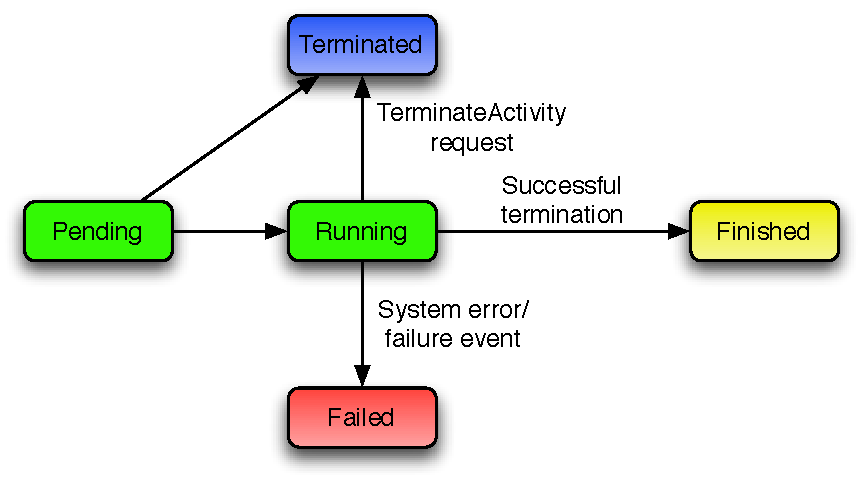
\includegraphics[scale=.75]{bes-basic-job-model}
  \end{center}
  \caption[Basic BES Job-State-Model]{This is the job-state-model as it is
    defined in the BES specification \cite{ogsa-bes}}
  \label{fig:bes-basic}
\end{figure}

A real  application can  specialize this state-model  for its own  use and
define new states and transitions as long as the \textbf{visual behaviour}
stays the same as of the basic state-model --- i.e.~no transitions must be
added that would not be allowed in the basic model.

The nice  thing about the extensibility  of this state-model  is, that any
client that  \emph{understands} the basic model,  will understand extended
model as  well, that  is because  the outer behaviour  did not  change and
therefore ``nothing unexpected'' ever happens.

\subsubsection{Extensions to the BES state-model}

Since the basic  \gls{glo:BES} state-model is a very  minimal one, we need
to  extend   it  to  allow   the  description  of   data-transfer  states.
Fortunately,  the \gls{glo:BES}  provides such  an extended  model  in its
specification, it is shown in Figure~\ref{fig:bes-extended}.

\begin{figure}
  \begin{center}
    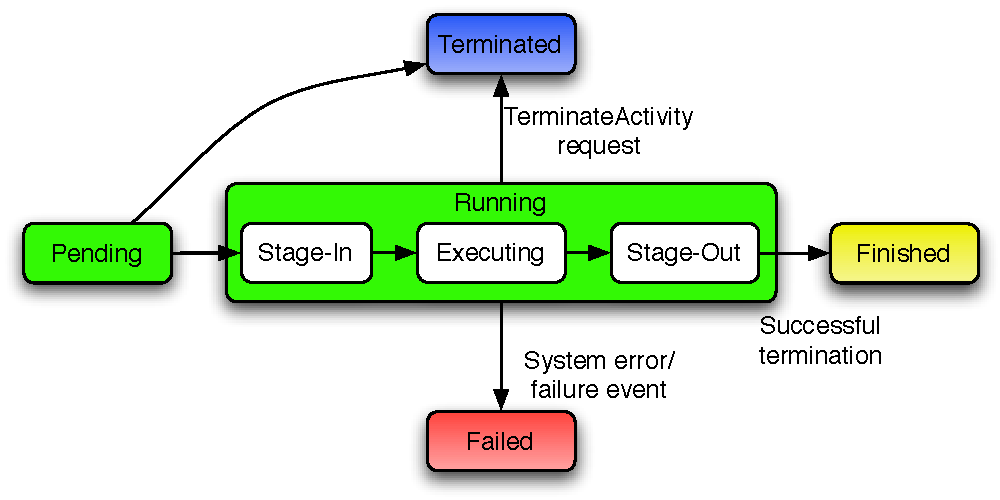
\includegraphics[scale=.75]{bes-staging-job-model}
  \end{center}
  \caption[BES State Model Staging Extension]{The basic BES state-model
    extended with sub-states to describe data-transfers.}
  \label{fig:bes-extended}
\end{figure}

The  \texttt{Running}   state  has   been  split  into   three  sub-states
\texttt{Stage-In}, \texttt{Stage-Out} and \texttt{Executing} --- the first
two describe data-transfer operations and the last one describes the state
in which the task is  actually being executed.  An invalid specialization,
for  example,  would   have  been  the  addition  of   a  transition  from
\texttt{Running:Stage-In} back  to \texttt{Pending}, since  that behaviour
is impossible in the basic state-model.

The  \gls{glo:BES}  specification  as  it  is for  the  JSDL,  defines  an
XML-Schema,  that is  to  be  used for  state  description. The  following
example shows  you the usage  of the state  description using XML  and how
specialized sub-states are represented. The main state is \texttt{Running}
and is  described using the \emph{ActivityStatus}  element, any sub-state,
that may currently be active,  depends on the application and therefore is
described using one or more elements from a different namespace.

\begin{minipage}{0.75\textwidth}
  \begin{lstlisting}[language=XML]
    <bes:ActivityStatus state="Running">
       <n00:Stage-In/>
    </bes:ActivityStatus>
  \end{lstlisting}
\end{minipage}

The example  makes use of  the previously defined  specialized state-model
and  describes an  activity  that is  currently  in the  \texttt{Stage-In}
sub-state of \texttt{Running} --- i.e.~it is waiting for its input data to
be  ready.  Any  client  which  is  not  aware  of  the  \texttt{Stage-In}
sub-state, will only ``see'' that  the activity is in the \texttt{Running}
state.


\subsection{Stopping tasks}
\label{sec:stopping-task}

As  you can  see in  Figure~\ref{fig:bes-extended}, each  non-terminal state
provides  a transition  to  the state  \texttt{Terminated}. That  directly
resembles the requirements for \emph{stopping a task} on user request.

In  case of  this work,  stopping  a task  may involve  shutting down  the
virtual  machine,  terminating active  data  transfers  and releasing  any
acquired resources.

\section{A more concrete concept}

This  section   outlines  a  more  concrete  concept   for  the  execution
environment and its  components. We are going to need  a component that is
responsible for  the requests a  user makes to the  execution environment,
this component  is also going to  manage the virtual machines  for each of
the tasks.

\begin{figure}[htbp]
  \begin{center}
    \begin{minipage}{.75\textwidth}
      \begin{center}
        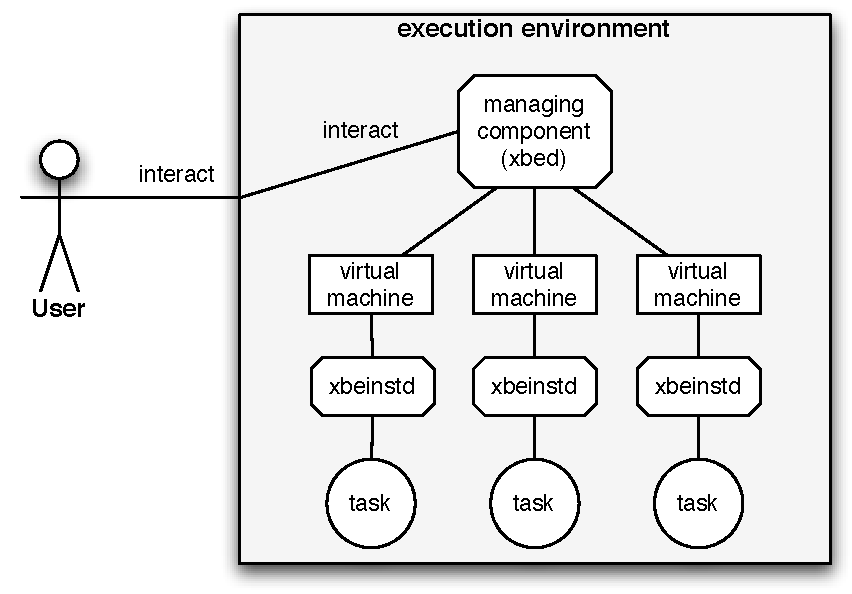
\includegraphics[scale=.5]{concrete-concept}
      \end{center}
      \caption[A  more  concrete  concept]{The  evolved concept,  using  a
        managing component to control  the virtual machines.  Each virtual
        machine  is   dedicated  to  a  single  task   submitted  by  some
        user. Users only interact with the managing component.}
      \label{fig:concrete-concept}
    \end{minipage}
  \end{center}
\end{figure}

Basically  this concept  defines a  client-server architecture,  where the
client is represented  by the user (or some mediator  such as a web-portal
or a  command-line client) and the  server is represented  by the managing
component.

The following  sections motivate the communication  architecture, which is
used  to connect up  clients and  the managing  component, and  a detailed
description of how the tasks should be handled.

\subsection{Basic communication architecture}
\label{sec:basic-communcation-architecture}

A  typical  way  of connecting  clients  with  some  server  is to  use  a
\gls{glo:TCP}-connection  to  the  server  for  each  client.   Since  the
communication which  takes place  in this environment  is message-oriented
--- as  you will  see later,  each request to  the server  is mapped  to a
single  XML document  ---  we can  abstract  from a  direct connection  to
logical  connection.  This logical  connection  can  be established  using
so-called \emph{message queue servers} (\gls{glo:MQS}).

\gls{glo:MQS}   have  several  very   important  advantages   over  direct
connections between the clients and the server:

\begin{itemize}
\item All messages are  sent to \textbf{logical queues} (i.e.~end-points),
  that  means   that  the  physical  address  (e.g.~IP   address)  of  any
  participating  service  (be  it  the  server or  a  client)  may  change
  unnoticeable to the communication partner.
\item All connections are  \textbf{outbound}, which effectively means that
  the server may also reside behind a firewall or a \gls{glo:NAT}-gateway.
  This not only increases the security  of the server (in means of allowed
  inbound  connections),  but  also  targets the  problems  which  typical
  network-policies and  resulting network-layouts of  grid-environments or
  companies impose.
\item The  \gls{glo:MQS} need not  to be on  a single machine, but  can be
  distributed  over  many computers  to  implement \textbf{fail-over}  and
  \textbf{load-balancing}.
\item  Messages are  stored within  the \gls{glo:MQS},  if they  cannot be
  delivered right now.   That may happen, if the  communication partner is
  temporarily disconnected  --- all pending messages will  be delivered as
  soon as the end-point connects again.
\item Multiple  \gls{glo:MQS} can be  configured to provide  forwarding of
  messages  destined for a  particular queue  --- that  means independence
  from the actual network-topology.
\item A \gls{glo:MQS} can be configured to provide \textbf{authentication}
  and \textbf{authorization} to limit  access to (i.e.~send to and receive
  from) particular queues.
\end{itemize}

\begin{figure}[htbp]
  \begin{center}
    \begin{minipage}{.75\textwidth}
      \begin{center}
        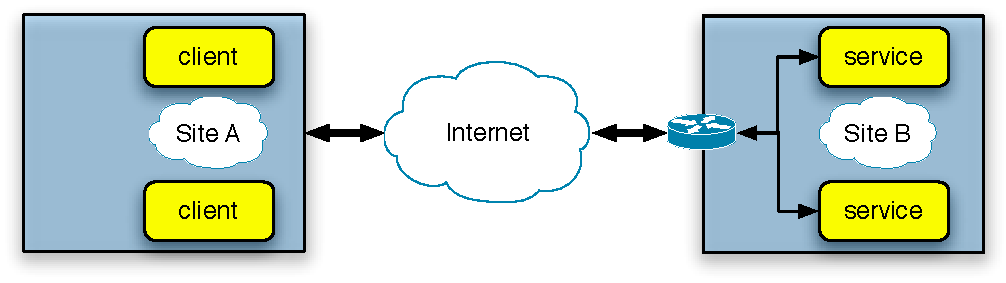
\includegraphics[scale=.5]{mqs-topology}
      \end{center}
      \caption[Example MQS topology]{A simple message-oriented system
        which is using a \gls{glo:MQS}.}
      \label{fig:mqs-topology}
    \end{minipage}
  \end{center}
\end{figure}

As you can see in  Figure~\ref{fig:mqs-topology}, site B has some services
connected to  a \gls{glo:MQS}.  These services can  be reached  by clients
from site A through an internet connection. The steps involved in building
up this communication scheme are:
\begin{enumerate}
\item  Each service  connects to  the \gls{glo:MQS}  and \emph{subscribes}
  itself to a unique queue (e.g.~service.\emph{X}).
\item    Clients   subscribe    themselves   to    unique    queues,   too
  (e.g.~client.\emph{Y}).
\end{enumerate}

Now  that each  party is  subscribed to  its own  unique queue,  a two-way
communication is possible:
\begin{enumerate}
\item A client  that wants to communicate with one  of the services, sends
  its messages  to the unique queue  of that particular  service. The sent
  message  contains a  \emph{reply-to} field  which is  set to  the unique
  queue of the client.
\item Answers from  a service to a connected client are  sent to the queue
  specified in the reply-to field of received messages.
\end{enumerate}

\section{Support for Calana}
\label{sec:calana-support}

\emph{Calana} is  a new  Grid-scheduler approach proposed  by M.~Dalheimer
\cite{dalheimer05agentbased}.  The  scheduler uses \emph{agents}  that are
responsible for  a single  resource and at  least one  \emph{broker}.  The
broker initiates an \emph{auction} among  the connected agents to assign a
task to some resource.

\begin{figure}[htbp]
  \begin{center}
    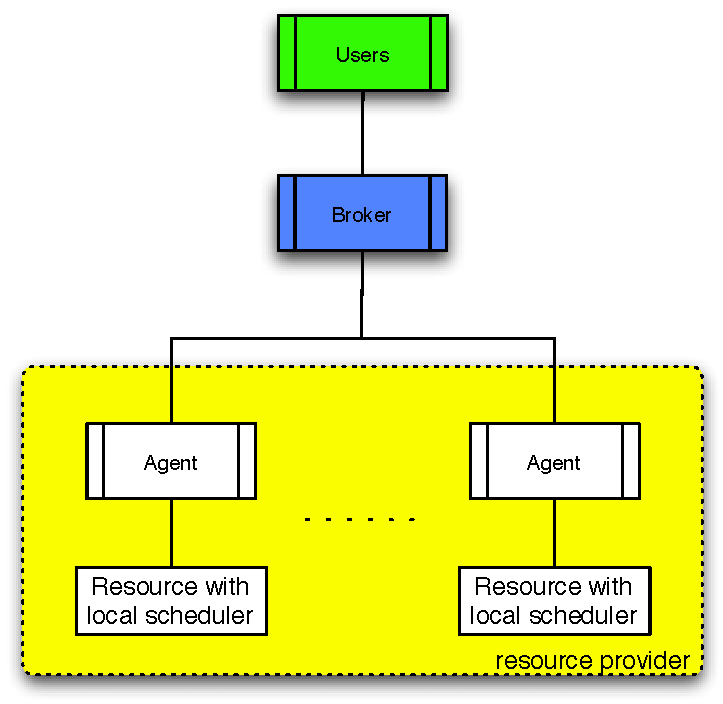
\includegraphics[scale=0.5]{calana-architecture}
  \end{center}
  \caption{Architecture of Calana}
  \label{fig:calana-architecture}
\end{figure}

An  abstract   view  over   the  architecture  of   Calana  is   shown  in
Figure~\ref{fig:calana-architecture}.   For a  detailed discussion  of the
Calana-protocol  that  is used  to  perform an  auction,  have  a look  at
\cite{dalheimer06calanaprotocol,petry06}, but  the  main steps  involved
are:
\begin{enumerate}
\item When a user submits a job to the Calana-broker, the broker will open
  up an auction and try to \emph{book} a resource for the task.
\item    For   each   task    an   auction    is   created    by   sending
  \texttt{BookingReq}-messages to the connected agents.
\item The agents will make  one or more \emph{reservations} on their local
  scheduler  and  answer with  a  \texttt{AuctionBid}.   Bids contain  for
  example  the  cost  of   using  the  resource  and  various  reservation
  parameters  such  as  the   earliest  start-time  and  duration  of  the
  reservation.
\item To make a decision, the  broker judges all received bids and chooses
  the     best     one      according     to     some     preference-model
  \cite{dalheimer05agentbased, petry06}.
\item If  the user  accepts the decision,  the broker  \emph{confirms} the
  reservation.
\end{enumerate}

To  support  Calana, the  \gls{glo:XenBEE}  must  provide some  additional
functionality. One of these functionalities is a mechanism to \emph{make},
\emph{cancel}   and   \emph{confirm}   reservations.   To   reflect   that
requirement, we discussed about a common state-model for the jobs and came
to the consensus of adopting the \gls{glo:BES} model to our needs.

The implementation of Calana, which is currently still in development, too
uses message queues to implement the communication between the brokers and
the agents.

\begin{figure}[htbp]
  \begin{center}
    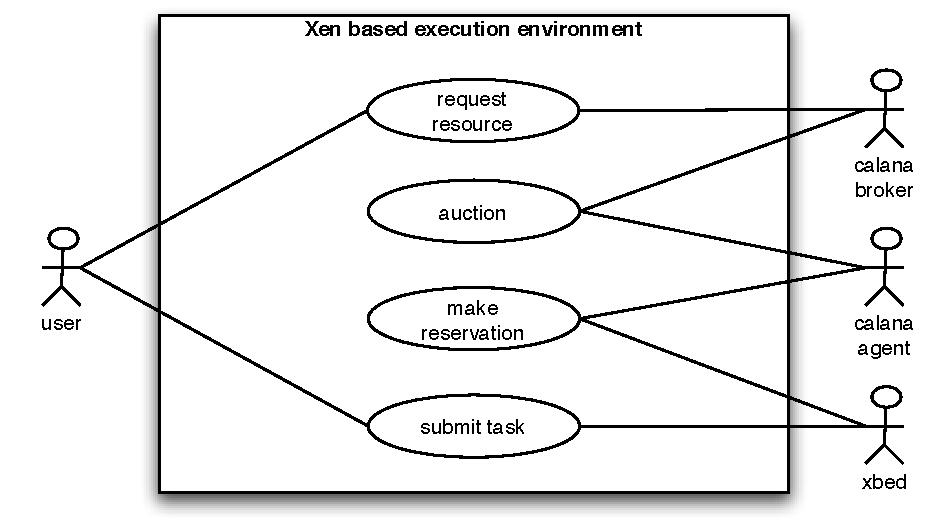
\includegraphics[scale=0.7]{uc-calana-xenbee}
  \end{center}
  \caption[Calana and  XenBEE]{The actors and use cases  that are involved
    when a Calana agent uses the \gls{glo:XenBEE} as its resource.}
  \label{fig:calana-xenbee}
\end{figure}

The picture  in Figure~\ref{fig:calana-xenbee} describes how  a user would
interact  with  a  system,  that   uses  Calana  for  scheduling  and  the
\gls{glo:XenBEE} as  its execution environment. The user  first requests a
resource from  the broker, who in turn  will open up an  auction among the
agents.   One of  those  agents are  shown  in the  figure,  he creates  a
reservation on the \emph{xbed} he  is attached to.  The user is eventually
presented  a unique identifier  for his  reservation which  he can  use to
submit his task to the \emph{xbed}.

\section{Use cases}
\label{sec:use-cases}

This section describes possible use cases for the \gls{glo:XenBEE}. I have
already shortly described, what the  basic requirements to this system are
and now  I am  going to show  you some  use cases and  which parts  of the
architecture are involved in each of them.

The ``big picture'' is shown in Figure~\ref{fig:system-usecases}, it shows
a compendium  of several possible  use cases from  a very high  level. The
involved    actors    are     the    \emph{user},    the    \emph{managing
  component}\footnote{denoted as \emph{xbed} --- the ``Xen-based Execution
  Daemon''}     mentioned      earlier     and     a      new     managing
component\footnote{denoted   as   \emph{xbeinstd}   ---  the   ``Xen-based
  Execution Instance Daemon''} which  is running on and solely responsible
for a single virtual machine.

\begin{figure}[htbp]
  \begin{center}
    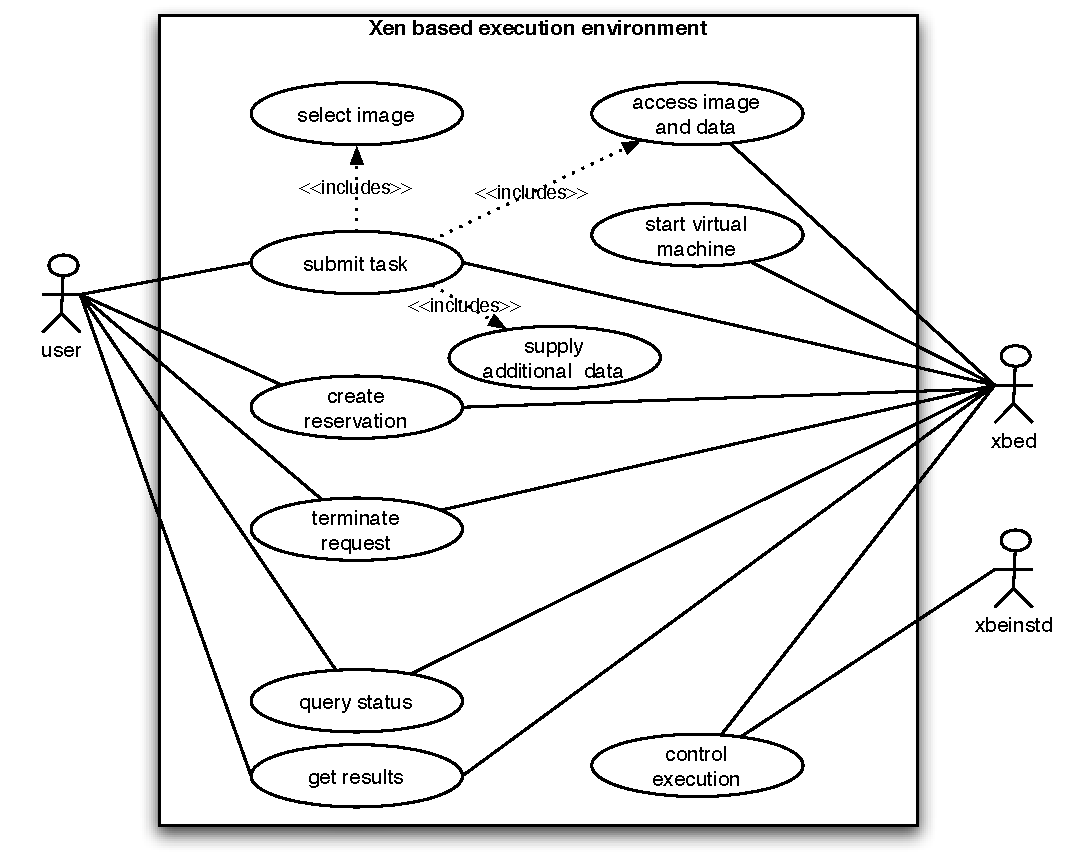
\includegraphics[scale=0.7]{system-usecase}
  \end{center}
  \caption[Use case  overview]{An overview  of several possible  use cases
    and the involved actors.}
  \label{fig:system-usecases}
\end{figure}


\subsection{Task submission}
\label{sec:uc-task-submission}

The very  first use case is  the submission of a  \emph{simple} task. With
\emph{simple} I mean, that the  task does not require any additional data,
it just  requires a previously prepared \gls{glo:image}  that contains the
application and the \emph{xbeinstd}.

On  server-side, the  \emph{xbed}  will associate  the  submission with  a
previously acquired  reservation ---  i.e.~the user creates  a reservation
first  which results in  some kind  of handle  (a unique  identifier which
refers to the  reservation) and then the user submits  his task using that
reservation.

\begin{figure}[htbp]
  \begin{center}
    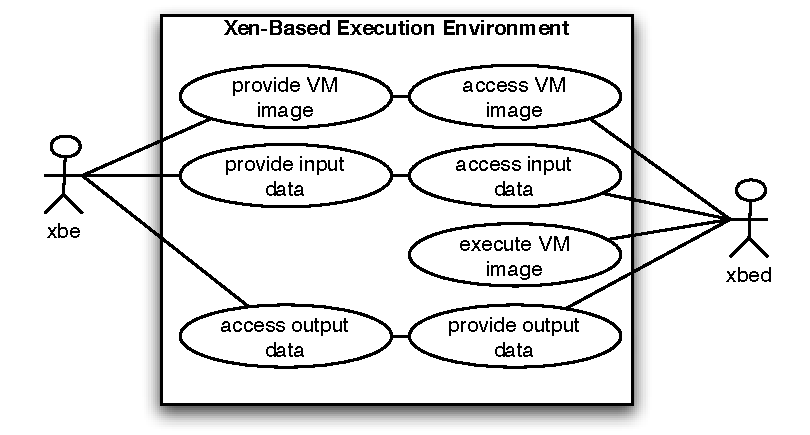
\includegraphics[scale=.75]{uc-submit-task}
  \end{center}
  \caption[UC Task submission]{Actors involved  in the task submission use
    case.}
  \label{fig:uc-submit-task}
\end{figure}

\paragraph{Selecting an image}
In  Figure~\ref{fig:uc-submit-task} the  required steps  for  submitting a
task are  shown. The  submission of  a task includes  the selection  of an
image  that  contains  the  application  the user  wants  to  execute.   A
sophisticated process of image-selection  can be rather complicated, since
it involves matching of available images against a description provided by
the user. Such  selection mechanisms are out of the  scope of this thesis,
but  in  a  later  use  case,  server-side  \emph{caching  of  data}  (see
Section~\ref{sec:uc-data-caching}),  a  simple way  of  selection will  be
described.

\paragraph{Accessing the image}
After the user submitted a  task, the \emph{xbed} has to \emph{access} the
specified image,  i.e.~the \emph{xbed} will initiate the  retrieval of the
image.   The  location  of  the  image  can for  example  be  given  as  a
\gls{glo:URI}  to   provide  an  uniform  and   extensible  mechanism  for
describing data locations.

If errors occur  during the image retrieval, the  \emph{xbed} has to abort
the task execution and must inform the user about the failure.

\subsection{Data staging}
\label{sec:uc-data-staging}

This  use case  is an  enhancements  over the  previous one,  it not  only
involves the  submission of an image,  but also the  specification of data
that  must  be  available  prior  executing  the task  and  that  must  be
transfered back to user after the task has finished.

\begin{figure}[htbp]
  \begin{center}
    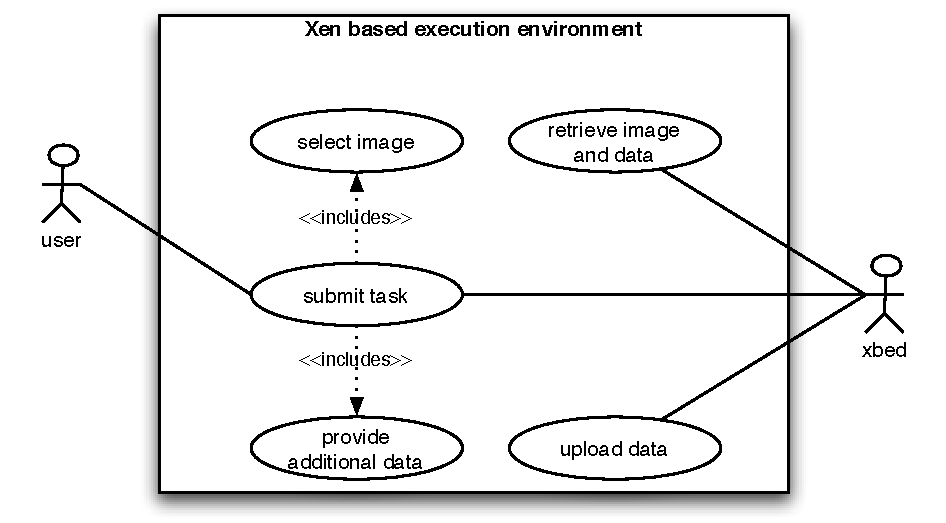
\includegraphics[scale=.75]{uc-data-staging}
  \end{center}
  \caption[UC  Data  Staging]{A user  submitting  a  task with  additional
    data.}
  \label{fig:uc-data-staging}
\end{figure}

Again,  the JSDL comes  into play  here, because  it already  supports the
description of staging operations. The \emph{xbed} has now to retrieve not
only  the image  file, but  also  all the  additional files  the user  has
specified to be staged in.

After the job  has finished its execution, the  \emph{xbed} is responsible
for staging  out generated  files. Therefore the  user must  specify which
files that are and to which locations they have to be uploaded. Source and
destination locations of files can again be specified as \gls{glo:URI}s.

\subsection{On-demand VM-deployment}
\label{sec:uc-on-demand-vm-deployment}

Well, this use  case can be seen  as a variant of the  task submission use
case. The purpose of this use case is the creation of a virtual machine on
user request without executing any task.

The resulting virtual  machine could be accessed by  the user through some
remote mechanism such as \gls{glo:SSH} \cite{openssh}.  With \gls{glo:SSH}
the user gains full control over his created virtual machine and can setup
and install any application he likes.

The login  to the  VM can  be provided using  public-keys that  are either
previously  installed  into the  image  or  uploaded  later on  using  the
standard   stage-in   process  (please   consult   the  documentation   on
\gls{glo:SSH} for more information about public-key authorization).


\subsection{Caching of data}
\label{sec:uc-data-caching}

Imagine a user,  who wants to execute the  same application several times.
That would mean he has to submit the same image over and over again, which
imposes a heavy load on the network connecting user and provider (i.e. the
host on which the \emph{xbed} runs). It would be wise to provide a caching
mechanism, that  allows the  user to store  his image on  server-side. The
caching efficiently  reduces network load and  decreases overall execution
time \cite{locality-principle}.

\begin{figure}[h]
  \begin{center}
    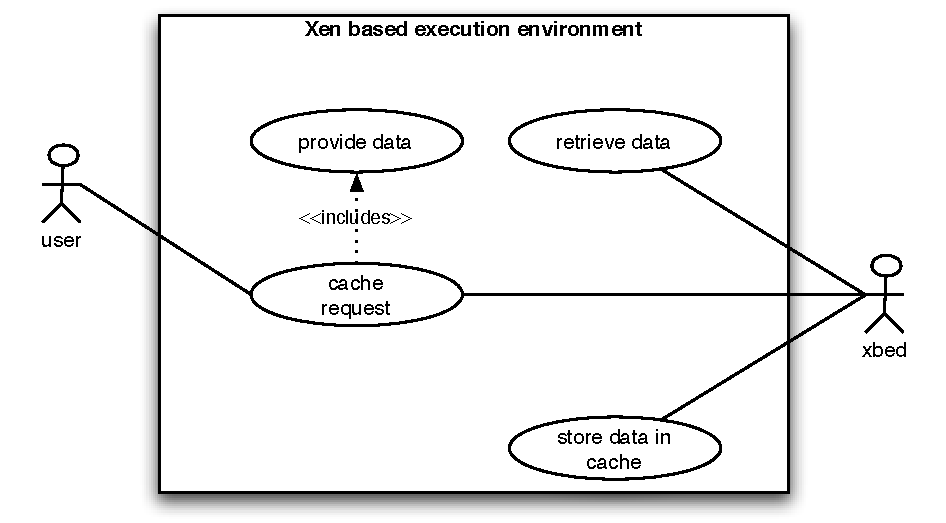
\includegraphics[scale=.75]{uc-data-caching}
  \end{center}
  \caption[UC  Data  Caching]{A user  who  is  requesting  the caching  of
    (arbitrary) data.}
  \label{fig:uc-data-caching}
\end{figure}

In  Figure~\ref{fig:uc-data-caching} the required  steps for  caching some
data are  shown. The user  makes his request  for caching the data  to the
\emph{xbed}, which in turn retrieves the data and stores it in a cache. To
make  the ``discovery''  of cached  data easier  for the  users,  the user
should be required to give some descriptive information for the data he is
going to  cache. As the return of  the request, the user  should receive a
unique identifier or an \gls{glo:URI} for the created entry in the cache.

The details  of how  exactly the caching  works are  highly implementation
specific, the most important point is  how the cached data can be referred
to by users of the system at a later point in time.

\paragraph{Referencing cached  data}

Cached data must be referable by the user for subsequent task submissions.
Since the submission of tasks uses \gls{glo:URI}s to indicate the location
of a  file, an obvious  way is  to use a  \gls{glo:URI} here as  well. The
caching of some data should  therefore result in a \gls{glo:URI}, that the
user can use in his job and staging descriptions.

\begin{figure}[h!]
  \begin{center}
    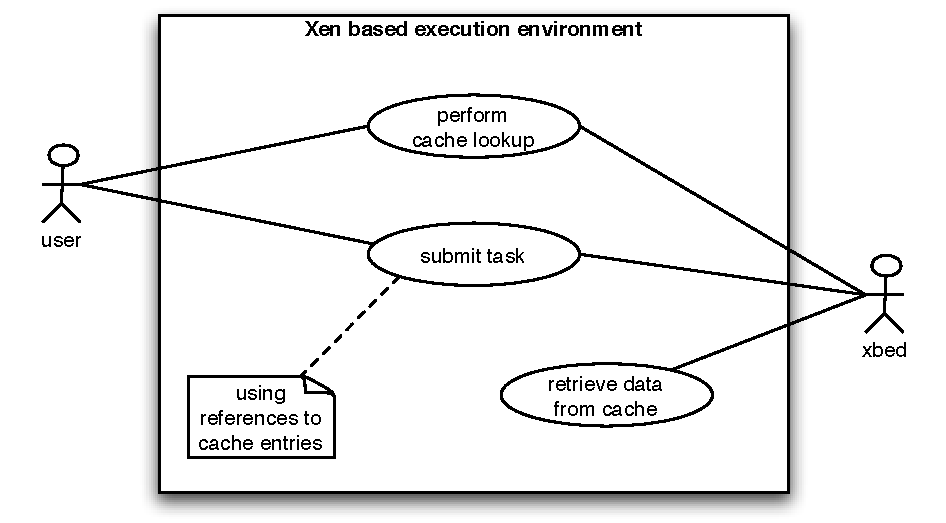
\includegraphics[scale=.75]{uc-cache-lookup}
  \end{center}
  \caption[UC  Cache Lookup]{A user  who  is using cached entries within
    his task submission.}
  \label{fig:uc-cache-lookup}
\end{figure}

Additionally, a really  nice thing to have in this  situation is some kind
of a lookup mechanism for cached  entries --- i.e.~a user does not need to
remember all the  \gls{glo:URI}s his entries have, but can  use a query to
the    system   and   thus    figure   out,    which   cache    entry   to
use. Figure~\ref{fig:uc-cache-lookup} shows you  how a user looks up cache
entries and uses them in a subsequent task submission.

\subsection{Terminating a task}
\label{sec:uc-terminate-task}

As   you   could   see   in   the   \gls{glo:BES}   job   state-model   in
Figure~\ref{fig:bes-extended},  the  user  must  have the  possibility  to
terminate his  submitted task at any  time and no matter  what the current
state of the task is.

\begin{figure}[h!]
  \begin{center}
    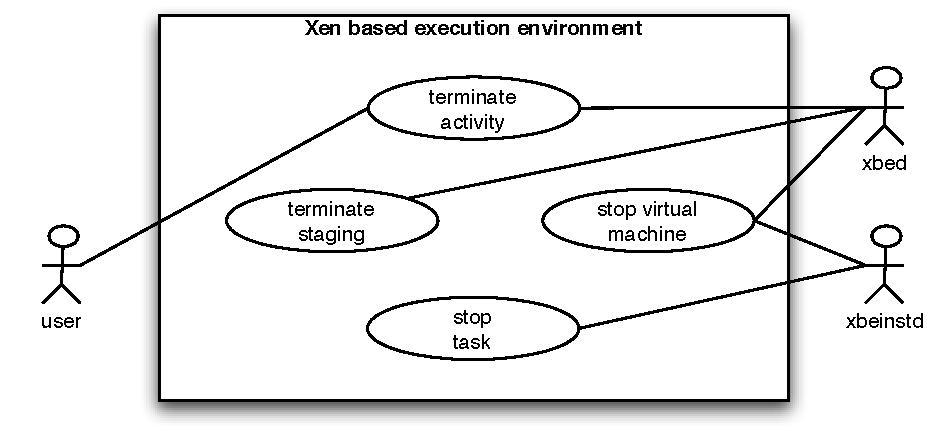
\includegraphics[scale=.75]{uc-terminate-task}
  \end{center}
  \caption[UC Terminate Task]{A user  who is requesting the termination of
    his  submitted task  and possible  use cases  that may  then  arise on
    server-side.}
  \label{fig:uc-terminate-task}
\end{figure}

The termination request  for a task can be received in  any state and that
may require  additional actions to be  taken in the  \emph{xbed}.  If, for
instance,  a virtual  machine has  already been  created and  is currently
executing the user's task, the application and the virtual machine have to
be terminated, too.  The same  holds for staging activities, that could be
currently active, they  have to be terminated cleanly  as well.  These use
cases are  shown in  Figure~\ref{fig:uc-terminate-task}. As you  can seen,
the \emph{xbeinstd} may be involved again, since the actual execution of a
task falls within his responsibility.

\subsection{Providing encrypted data}
\label{sec:uc-ecrypted-data}

Since all  data is referred to  by \gls{glo:URI}s, that  may be accessible
not  only  from  the  \emph{xbed}  itself, but  also  from  other  sources
(i.e.~probably unknown and  hostile ones), it is desirable  to store those
files encrypted. Of  course, if a user stores  an encrypted image-file and
wants  the \emph{xbed} to  use it  for execution,  the image-file  must be
decrypted on server-side prior booting a virtual machine with it.

\begin{figure}[h!]
  \begin{center}
    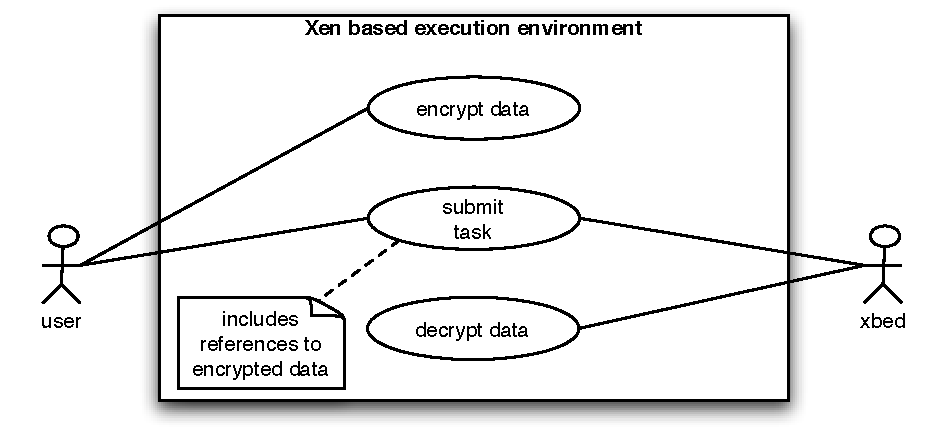
\includegraphics[scale=.75]{uc-encrypted-data}
  \end{center}
  \caption[UC  Encrypted  Data]{Submission   of  encrypted  data  and  its
    decryption prior execution by the \emph{xbed}.}
  \label{fig:uc-terminate-task}
\end{figure}

\section{Security issues}
\label{sec:security-requirements}

The proposed system  will use message queues to  transfer messages between
clients and the server, that means  all messages that are sent can be read
by any person or system in between any two communication partners. 

A   typical  solution   to  make   the  transfer   secure  is   using  the
\emph{Transport Layer  Security} protocol --- or  \gls{glo:TLS} for short.
\gls{glo:TLS} makes sure that  traffic between two endpoints is transfered
securely (i.e.~no eavesdropping, modification or message forgery).

\subsubsection{Transport Layer Security (TLS)}


\subsubsection{Message Layer Security (MLS)}

%%% Local Variables: 
%%% mode: latex
%%% TeX-master: "main.tex"
%%% End: 
